\documentclass[aspectratio=169]{beamer}
% Shared preamble for ml/ slide decks.
% Each lecture .tex starts with:
%   \documentclass[aspectratio=169]{beamer}
%   \input{../preamble}
% Compile from inside the chapter folder so \input{../preamble} resolves.

\usetheme{default}
\usecolortheme{dove}

\setbeamertemplate{navigation symbols}{}
\setbeamertemplate{footline}{%
  \hfill{\large\insertframenumber\,/\,\inserttotalframenumber}\hspace{0.8em}\vspace{0.5em}%
}

% Project palette (existing, kept for backwards compatibility with deferred/*)
\definecolor{popblue}{RGB}{52, 101, 164}
\definecolor{sampred}{RGB}{204, 0, 0}
\definecolor{paramgreen}{RGB}{0, 140, 70}
\definecolor{warnred}{RGB}{180, 40, 40}
\definecolor{orange1}{RGB}{220, 120, 0}
\definecolor{violet1}{RGB}{120, 50, 160}
\definecolor{lightbg}{RGB}{245, 245, 250}

% Armenian flag palette (use these for any 3-color highlight; per CLAUDE.md).
% "Nice versions": slightly de-saturated from the official spec for slide use,
% so they don't burn out under projector colors. Originals kept as *_pure.
\definecolor{armred}{RGB}{200, 30, 40}      % nice red (official #D90012 muted)
\definecolor{armblue}{RGB}{30, 70, 160}     % nice blue (official #0033A0 muted)
\definecolor{armorange}{RGB}{230, 160, 30}  % nice orange (official #F2A800 muted)
\definecolor{armred_pure}{HTML}{D90012}     % official Armenian flag red
\definecolor{armblue_pure}{HTML}{0033A0}    % official Armenian flag blue
\definecolor{armorange_pure}{HTML}{F2A800}  % official Armenian flag orange

\setbeamercolor{frametitle}{fg=popblue}
\setbeamercolor{title}{fg=popblue}

\usepackage{pgfplots}
\usepackage{tikz}
\usetikzlibrary{shapes, arrows.meta, positioning, calc, decorations.pathreplacing, patterns, matrix}
\pgfplotsset{compat=1.18}
\usepackage{amsmath, amssymb, amsfonts}
\usepackage{bm}
\usepackage{dsfont}
\usepackage{array}
\usepackage{pifont}
\usepackage{colortbl}
\usepackage{fontenc}

% Callout boxes. Purely additive - existing decks are unaffected.
% Usage: \begin{tcolorbox}[colback=armblue!8, colframe=armblue, boxrule=0.6pt, arc=2pt,
%                          title=\textbf{Key idea}] ... \end{tcolorbox}
% Palette convention (ml/SLIDE_STYLE.md): armblue=key idea, armred=trap/warning,
% paramgreen=takeaway or "Next", armorange=watch-out.
\usepackage[most]{tcolorbox}

% Cleaner table rules (\toprule, \midrule, \bottomrule). Also purely additive.
\usepackage{booktabs}

% \cancel{...} for struck-through terms in derivations (added 2026-08-11 for the
% importance-sampling frame in ch11_rl, where the dynamics cancel). Purely additive.
\usepackage{cancel}

% Minimal ML notation macros (subset of slds-lmu latex-math/basic-ml.tex).
% Kept here so we don't have to inline-expand every \thetav, \xv, etc.
% when porting upstream slides.
\newcommand{\R}{\mathds{R}}
\newcommand{\N}{\mathds{N}}
\newcommand{\E}{\mathds{E}}
\newcommand{\Xspace}{\mathcal{X}}
\newcommand{\Yspace}{\mathcal{Y}}
\newcommand{\Hspace}{\mathcal{H}}
\newcommand{\D}{\mathcal{D}}
\newcommand{\Dtrain}{\mathcal{D}_{\text{train}}}
\newcommand{\Dtest}{\mathcal{D}_{\text{test}}}
\newcommand{\xv}{\mathbf{x}}
\newcommand{\yv}{\mathbf{y}}
\newcommand{\Xmat}{\mathbf{X}}
\newcommand{\id}{\mathbf{I}}
\newcommand{\thetav}{\bm{\theta}}
\newcommand{\thetah}{\hat{\bm{\theta}}}
\newcommand{\lamv}{\bm{\lambda}}
\newcommand{\fx}{f(\xv)}
\newcommand{\fxt}{f(\xv \,|\, \bm{\theta})}
\newcommand{\fxi}{f\!\left(\xv^{(i)}\right)}
\newcommand{\fh}{\hat{f}}
\newcommand{\fxh}{\hat{f}(\xv)}
\newcommand{\yh}{\hat{y}}
\newcommand{\yih}{\hat{y}^{(i)}}
% \xi clashes with the Greek letter \xi; write \xv^{(i)} inline instead.
\newcommand{\yi}[1][i]{y^{(#1)}}
\newcommand{\xyi}[1][i]{\left(\xv^{(#1)},\, y^{(#1)}\right)}
\newcommand{\thx}{\bm{\theta}^\top \xv}
\newcommand{\sumin}{\sum_{i=1}^{n}}
\newcommand{\sumjp}{\sum_{j=1}^{p}}
\newcommand{\Lxy}{L\!\left(y, \fx\right)}
\newcommand{\Lxyi}{L\!\left(\yi, \fxi\right)}
\newcommand{\risk}{\mathcal{R}}
\newcommand{\riske}{\mathcal{R}_{\text{emp}}}
\newcommand{\risket}{\mathcal{R}_{\text{emp}}(\bm{\theta})}
\newcommand{\riskt}{\mathcal{R}(\bm{\theta})}
\newcommand{\riskr}{\mathcal{R}_{\text{reg}}}
\newcommand{\argmin}{\mathop{\mathrm{arg\,min}}}
\newcommand{\argmax}{\mathop{\mathrm{arg\,max}}}
\newcommand{\eps}{\varepsilon}


\graphicspath{{fig/}{../00_shared/fig/}{../00_shared/fig/borrowed/}{../00_shared/fig/borrowed/3b1b/}{../00_shared/fig/borrowed/paper/}}

% credit / citation lines (as in LLM-3)
\newcommand{\bbb}{{\scriptsize\color{gray} 3Blue1Brown}}
\newcommand{\paper}[1]{{\scriptsize\color{gray} #1}}
\newcommand{\src}[1]{{\scriptsize\color{gray} #1}}
\newcommand{\link}[2]{\href{#1}{\textcolor{popblue}{#2}}}   % no underline: long titles must break

% full-bleed 3Blue1Brown still with a one-line caption pinned near the bottom. Wrapped in a group
% so the background template reverts after this one [plain] frame. Needs 2 pdflatex passes.
\newcommand{\bbbcap}[2]{%
  {\usebackgroundtemplate{\includegraphics[width=\paperwidth,height=\paperheight]{#1}}%
  \begin{frame}[plain]
    \begin{tikzpicture}[remember picture, overlay]
      \node[anchor=south west, font=\tiny, text=white!60]
        at ([shift={(0.26cm,0.16cm)}]current page.south west) {3Blue1Brown};
      \node[anchor=south, font=\small\itshape, text=white, fill=black!60,
            inner sep=5pt, rounded corners, text width=0.86\paperwidth, align=center]
        at ([shift={(0,0.85cm)}]current page.south) {#2};
    \end{tikzpicture}
  \end{frame}}%
}

% callout boxes, matching LLM-1, LLM-2, LLM-3 and LLM-6
\newcommand{\keybox}[1]{\fcolorbox{armblue}{armblue!8}{\parbox{0.97\linewidth}{\small #1}}}
\newcommand{\trapbox}[1]{\fcolorbox{armred}{armred!8}{\parbox{0.97\linewidth}{\small #1}}}
\newcommand{\takebox}[1]{\fcolorbox{paramgreen}{paramgreen!8}{\parbox{0.97\linewidth}{\small #1}}}
\newcommand{\watchbox}[1]{\fcolorbox{armorange}{armorange!12}{\parbox{0.97\linewidth}{\small #1}}}

\newcommand{\sectiontransition}[2]{%
  \begin{frame}[plain]
    \vfill
    \begin{center}
      {\Huge\bfseries\color{popblue} #1}\\[1.1em]
      {\large #2}
    \end{center}
    \vfill
  \end{frame}}

\title{The Transformer block}
\subtitle{Many heads, the MLP, and the residual stream}
\author{}
\date{}

\begin{document}

\begin{frame}[plain]
  \titlepage
  \begin{center}\scriptsize\color{gray}
    LLM chapter, session 4. Parts adapt 3Blue1Brown, ``Deep Learning'' chapters 6 and 7.
  \end{center}
\end{frame}

% ============================================================ LINKS (2026-10-27, as in LLM-1 to LLM-3)
\begin{frame}{Before we start: two videos and a demo}
  \begin{columns}[T]
    \column{0.49\textwidth}
    \keybox{\raggedright\textbf{Recommended viewing}\\[4pt]
    3Blue1Brown, \link{https://www.youtube.com/watch?v=9-Jl0dxWQs8}{How might LLMs store facts
    \textbar{} Deep Learning Chapter 7} (2024, 23 min): today's MLP section, animated - the
    Michael Jordan stills are from it.\\[6pt]
    Andrej Karpathy, \link{https://youtu.be/kCc8FmEb1nY?t=4919}{Let's build GPT: from scratch, in
    code, spelled out.} (2023). From 1:21:59: many heads, the MLP, residual connections and
    LayerNorm, added to a working model one at a time.}
    \column{0.49\textwidth}
    \takebox{\raggedright\textbf{Live demo:}
    \link{https://poloclub.github.io/transformer-explainer/}{Transformer Explainer} (LLM-3's)\\[4pt]
    Today, open the parts LLM-3 skipped: the 12 heads side by side, the MLP with its 3,072
    neurons, the residual add, LayerNorm.}
    \vskip 4pt
    {\small\textbf{Try:}}
    \begin{itemize}\small
      \item find a head that looks one token back
      \item find a head that parks on the first token
      \item follow one token through a whole block
    \end{itemize}
  \end{columns}
\end{frame}

% ============================================================ WHERE WE ARE (py_src/llm_roadmap.py)
\begin{frame}{Where we are: one forward pass}
  \begin{center}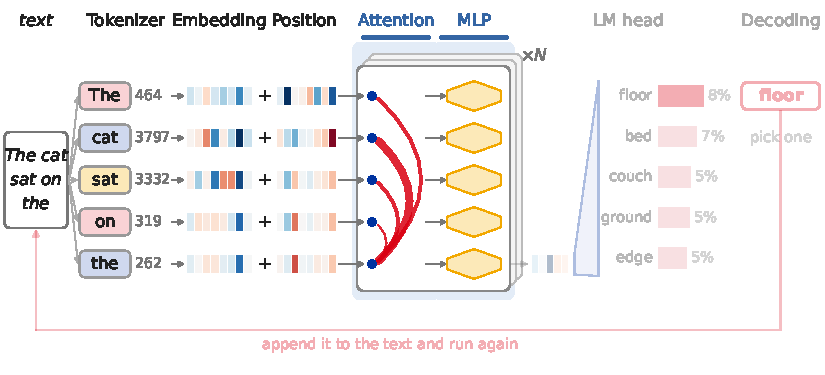
\includegraphics[width=\linewidth]{roadmap_block_pass.pdf}\end{center}
  \vskip -2pt
  {\small Today: the rest of one layer - many heads and the MLP - and why it stacks 12 times.}
\end{frame}

\begin{frame}{Where we are: the life of a model}
  \begin{center}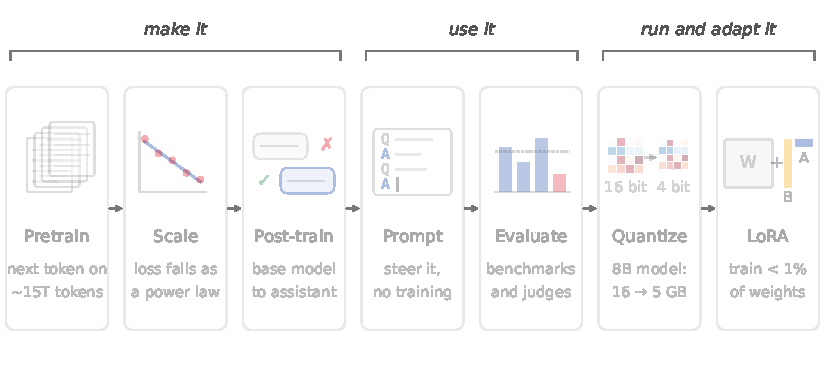
\includegraphics[width=\linewidth]{roadmap_block_life.pdf}\end{center}
  \vskip -2pt
  {\small Later: where these weights come from, and what you do with them once you have them.}
\end{frame}

% ============================================================ COLD OPEN
\begin{frame}{What does GPT-2 write next?}
  \vskip 6pt
  Four prompts for GPT-2 small, the model on our map. Predict its next word:
  \vskip 10pt
  \begin{center}
  \begin{tabular}{l}
    ``Lionel Messi plays the sport of \ldots'' \\[4pt]
    ``Henrikh Mkhitaryan plays the sport of \ldots'' \\[4pt]
    ``Ella Fitzgerald was a famous American \ldots'' \\[4pt]
    ``Elliott Smith was a famous American \ldots'' \\
  \end{tabular}
  \end{center}
  \vskip 12pt
  \keybox{\textbf{Predict:} which of the four does it get right? And for the ones it gets wrong,
  what does it say instead?}
\end{frame}

\begin{frame}{Stored, half-stored, missing}
  \begin{center}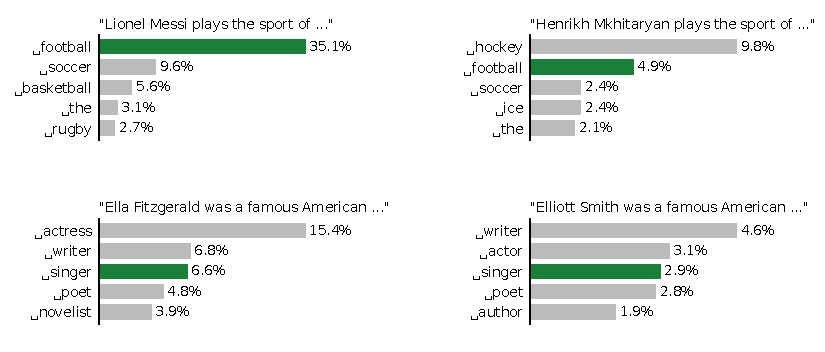
\includegraphics[width=0.94\linewidth]{blk_fact_probes.pdf}\end{center}
  \vskip -4pt
  {\small Messi is stored: football, 35\%. Mkhitaryan is missing: hockey first, football 5\%.
  ``Singer'' is third for both musicians, but 6.6\% against 2.9\%. One run of the real GPT-2.}
\end{frame}

\begin{frame}{So where does a fact live?}
  \vskip 10pt
  No word in these sentences says ``football'' or ``singer''.
  \vskip 8pt
  So the fact must come from the \textbf{weights} somewhere: a token's own row of the table
  (LLM-2), attention's matrices ($W_V$ and $W_O$ can write new directions too), or the other half
  of each layer, which LLM-3 never touched.
  \vskip 8pt
  And LLM-1 shows up again: ``Lionel Messi'' is 2 tokens, ``Henrikh Mkhitaryan'' is 7 pieces.
  The model has to put the name together before it can look anything up.
  \vskip 12pt
  \keybox{Today's answer, as far as the evidence goes: mostly in that other half, the
  \textbf{MLP} - and it is the bigger half. The evidence comes at the end of the MLP section.}
\end{frame}

\begin{frame}{Three things stand between one head and GPT-2}
  \vskip 6pt
  LLM-3 built \textbf{one head}: queries, keys, values, $\mathrm{softmax}(QK^\top/\sqrt{d_k})V$.
  To get from there to one layer of GPT-2:
  \vskip 8pt
  \begin{enumerate}
    \item[\textbf{1.}] \textbf{One head asks one question.} $\to$ many heads.
    \item[\textbf{2.}] \textbf{Tokens talk, but never think alone.} $\to$ the MLP, where facts like
      Messi's sport seem to live.
    \item[\textbf{3.}] \textbf{One layer is not a network.} $\to$ the residual stream and its
      norms. (LLM-3's causal mask rides along inside every attention layer.)
  \end{enumerate}
  \vskip 10pt
  \keybox{The three fixes bolted onto one head of attention \emph{are} the Transformer block.}
\end{frame}

\begin{frame}{Outline}
  \tableofcontents
\end{frame}

% ============================================================ SECTION 1
\section{Many heads}
\sectiontransition{Many heads}{One head asks one question.}

\begin{frame}{By hand: two heads, two questions}
  \begin{columns}[T]
    \column{0.42\textwidth}
    \small
    LLM-3's toy, slots [adjective, fluffy, blue, noun].
    \vskip 4pt
    \textbf{Head 1} asks ``any adjectives?'' (LLM-3's head): weights $0.47, 0.47, 0.06$; it
    hands over fluffiness, $0.47$.
    \vskip 4pt
    \textbf{Head 2} asks ``what colour?'' (its key reads the blue slot): weights
    $0.11, 0.79, 0.11$; it hands over blueness, $0.79$.
    \column{0.56\textwidth}
    \vskip 6pt
    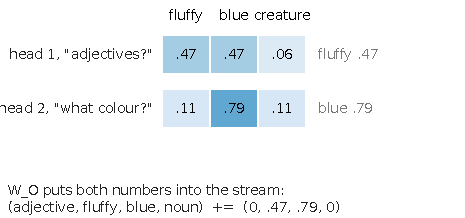
\includegraphics[width=\linewidth]{blk_two_heads.pdf}
  \end{columns}
  \vskip 6pt
  \takebox{Two questions at once, and two answers: $0.47$ and $0.79$. Real heads hand over 64
  numbers each, not one. (A new toy layer, so not LLM-3's result.)}
\end{frame}

\begin{frame}{By hand: $W_O$ puts the answers in the stream}
  \vskip 6pt
  Side by side, the two heads give $(0.47,\ 0.79)$. $W_O$ has one row per slot of the stream
  [adjective, fluffy, blue, noun] and one column per head's number:
  \[ W_O \begin{pmatrix}0.47\\0.79\end{pmatrix} =
     \begin{pmatrix}0&0\\1&0\\0&1\\0&0\end{pmatrix}\!\begin{pmatrix}0.47\\0.79\end{pmatrix}
     = \begin{pmatrix}0\\0.47\\0.79\\0\end{pmatrix} \]
  Head 1's number lands in the fluffy slot, head 2's in the blue slot; this update is added to
  creature's vector.
  \vskip 8pt
  \keybox{This toy $W_O$ only routes. A learned $W_O$ mixes: every row can take a little from
  every head, which is how 12 heads' answers become one 768-number update.}
\end{frame}

\begin{frame}{Run it $h$ times, in parallel}
  Nothing about one head changes. Learn $h$ independent sets of $W_Q, W_K, W_V$, run them at the
  same time, put the outputs side by side, and mix them with one more matrix $W_O$:
  \vskip 2pt
  \begin{center}
  $\text{MultiHead}(X) = \text{Concat}(\text{head}_1, \ldots, \text{head}_h)\, W_O$,
  \qquad $\text{head}_i = \text{Attention}(XW_Q^{(i)}, XW_K^{(i)}, XW_V^{(i)})$
  \end{center}
  \vskip 4pt
  \keybox{\textbf{GPT-2: 12 heads $\times$ 64 numbers $=$ 768}, the size of a token's vector
  (LLM-3's ``why 64''). Count: $12 \times 3 \times (768 \times 64) = 1{,}769{,}472 = 3 \times
  768^2$ - exactly one 768-wide head's $W_Q, W_K, W_V$, stored as one $768 \times 2{,}304$ matrix.
  $W_O$ adds $768 \times 768 = 589{,}824$, so every output number can draw on every head. Total
  $4 \times 768^2 = 2{,}359{,}296$, plus 3,072 biases: the 2,362,368 on the block chart later.}
  \vskip 2pt
  {\small Same weights as one 768-wide head: you \textbf{split} the budget, you do not add to it.
  What the split buys: one head gives each token \textbf{one} softmax, one way to weight the
  others; 12 heads give it 12 at once. They do not talk until the concatenation, so all twelve
  run as one batched matrix product, and they differ because they start from different random
  weights ([41]).}
\end{frame}

\bbbcap{multihead.png}{Multi-head attention: the same mechanism, many times over, each head free
to learn a different pattern. (3Blue1Brown draws GPT-3: 96 heads per layer. GPT-2 small has 12.)}

\begin{frame}{Do heads actually specialise, or is that a story?}
  \begin{columns}[T]
    \column{0.52\textwidth}
    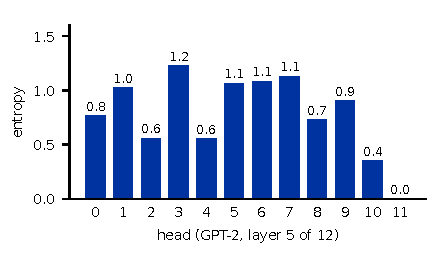
\includegraphics[width=\linewidth]{blk_gpt2_entropy.pdf}
    \column{0.46\textwidth}
    \vskip 6pt
    \small
    Measured: the real GPT-2, the creature sentence, the 12 heads of layer 5.
    \vskip 4pt
    \textbf{Attention entropy} $= -\sum_j a_{ij}\log a_{ij}$, averaged over rows. Reference
    points: 0 = all weight on one token; $\ln 2 = 0.69$ = split evenly over two; the more tokens
    it spreads over, the higher ($\ln 11 = 2.4$ for all 11).
    \vskip 4pt
    Head 11 scores \textbf{0.0}: every token puts all of its weight on a single token. Which one?
    Next slide.
  \end{columns}
\end{frame}

\begin{frame}{Three real heads, one sentence}
  \begin{center}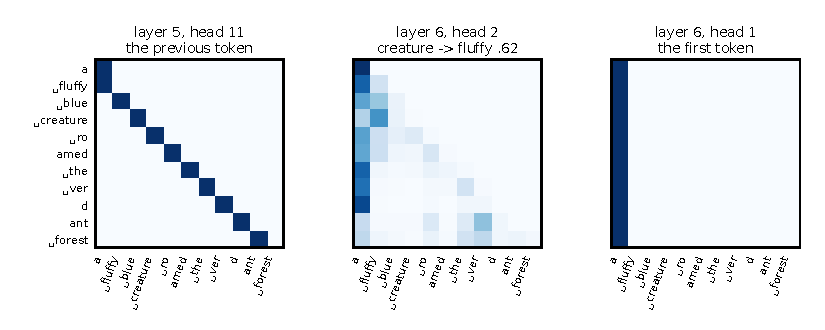
\includegraphics[width=\linewidth]{blk_gpt2_heads.pdf}\end{center}
  \vskip -6pt
  {\small Left: every token looks exactly one token back (weight 1.00) - the head with entropy 0.
  Middle: on this sentence, creature sends 62\% of its attention to fluffy - LLM-3's toy, for
  real. Right: everything goes to the first token, ``a''.}
\end{frame}

\begin{frame}{Attention sinks}
  \begin{columns}[T]
    \column{0.5\textwidth}
    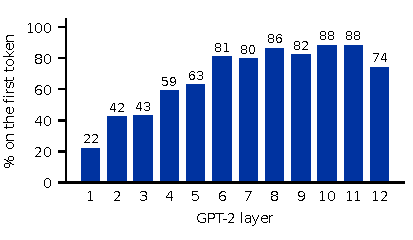
\includegraphics[width=\linewidth]{blk_gpt2_sink.pdf}
    \column{0.48\textwidth}
    \vskip 6pt
    \small
    The right-hand pattern is not rare: \textbf{39 of GPT-2's 144 heads} put over 90\% of their
    attention on the first token of this sentence. The share grows with depth: 22\% in layer 1,
    88\% in layer 10.
    \vskip 6pt
    The usual explanation: softmax must hand out a total of 1, so a head with nothing useful to
    look at parks its weight somewhere. The first token is the one place every later token can
    see (the mask), so the model learns to use it as the parking spot, and to keep what it
    hands over small.
  \end{columns}
  \vskip 6pt
  \watchbox{This is called an \textbf{attention sink} \paper{(Xiao et al., ICLR 2024)}. LLM-2 met
  its use: keep the first 4 tokens plus a window, and a model streams 4 million tokens. Real heads
  are messier than the toy, exactly as LLM-3 warned.}
\end{frame}

\begin{frame}{From quirk to design: letting a head look at nothing}
  \begin{itemize}
    \item Evan Miller (2023, a blog post, no experiments): add 1 to softmax's denominator, so the
      weights may sum to less than 1 and a head can attend to nothing. He called it ``Attention Is
      Off By One''.
    \item OpenAI's gpt-oss (2025) does a version of it: every head has a learned extra term in the
      softmax's denominator, ``which enables the attention mechanism to pay no attention to any
      tokens'' (model card).
    \item Qiu et al. (Qwen team, NeurIPS 2025 best paper): a learned gate on each head's output.
      Attention on the first token falls from 46.7\% to 4.8\% on average, and training gets more
      stable.
  \end{itemize}
  \vskip 6pt
  \takebox{A pattern first found by staring at attention grids became a line in 2025 model
  designs.}
\end{frame}

\begin{frame}{What the specialisations look like}
  \vskip 8pt
  Across models and layers, heads fall into recognisable jobs:
  \vskip 8pt
  \begin{center}
  \small
  \begin{tabular}{ll}
    \toprule
    \textbf{Kind of head} & \textbf{What it attends to} \\
    \midrule
    positional & the previous token, or the first one (both above) \\
    syntactic  & the verb belonging to this subject; the noun this adjective modifies \\
    coreference & the name a pronoun refers to \\
    lexical    & the other half of a multi-token name (\emph{Lionel} $\leftrightarrow$ \emph{Messi}) \\
    \bottomrule
  \end{tabular}
  \end{center}
  \vskip 10pt
  \watchbox{Read these labels with some suspicion. Nobody assigned these jobs; they are patterns
  \emph{we} recognise afterwards, on the sentences we looked at, and plenty of heads do nothing
  so tidy. The measured claim is that the heads differ.}
\end{frame}

\begin{frame}{Heads team up: the induction head}
  \begin{center}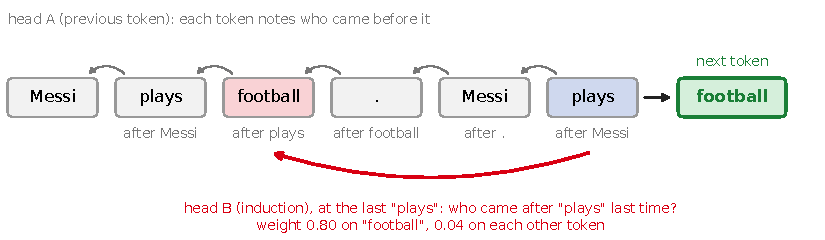
\includegraphics[width=0.9\linewidth]{blk_induction.pdf}\end{center}
  \vskip -6pt
  \begin{itemize}\small
    \item Head A writes ``who came before me'' into every token's vector. Head B's query is the
      current token; its keys read A's note; the best match is the token that followed ``plays''
      last time, and B copies it. \ldots\,A B\,\ldots\,A $\to$ B: \textbf{in-context learning},
      with nothing about Messi stored.
    \item Why two layers: heads in the same layer cannot read each other. B can only see A's note
      after A's output has been added to the stream, so A must sit in an earlier layer.
    \item Olsson et al. (2022) named these \textbf{induction heads}. They appear abruptly, early in
      training, at the same point where in-context learning jumps. Toy numbers here (a match
      scores 3); the interpretability chapter takes the real ones apart.
  \end{itemize}
\end{frame}

\begin{frame}{One head or twelve: still blind to order}
  \begin{center}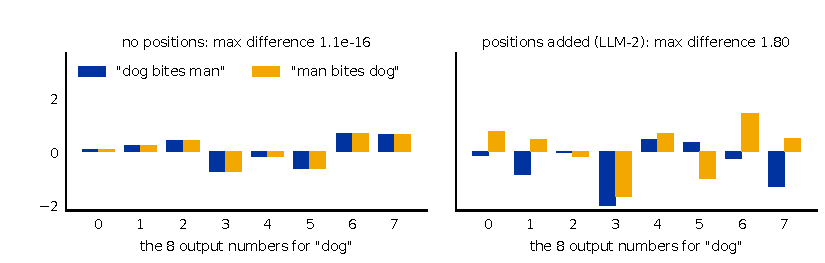
\includegraphics[width=0.92\linewidth]{blk_permutation.pdf}\end{center}
  \vskip -4pt
  {\small The proof LLM-2 promised. Same three word vectors, ``dog bites man'' vs ``man bites
  dog'', one head: ``dog'' gets the same output in both, up to $1.1 \times 10^{-16}$ -
  floating-point zero. Add positions (right) and the two differ.}
  \vskip 4pt
  \keybox{Nowhere for order to enter: $\mathbf{q}_i \cdot \mathbf{k}_j$ uses only the two
  vectors, softmax works on a set, and the output is a sum. Permute the inputs and the outputs
  come back permuted, unchanged. That is why LLM-2 adds positions before the first layer.}
\end{frame}

% ============================================================ SECTION 2
\section{The MLP: where facts live}
\sectiontransition{The MLP: where facts live}{Attention moves information around. Something has to
store it.}

\bbbcap{ch7_mj_hook.jpg}{3Blue1Brown's version of our question: ``Michael Jordan plays the sport
of \_\_\_''. Ours was Messi.}

\begin{frame}{Where the MLP sits}
  \begin{columns}[T]
    \column{0.56\textwidth}
    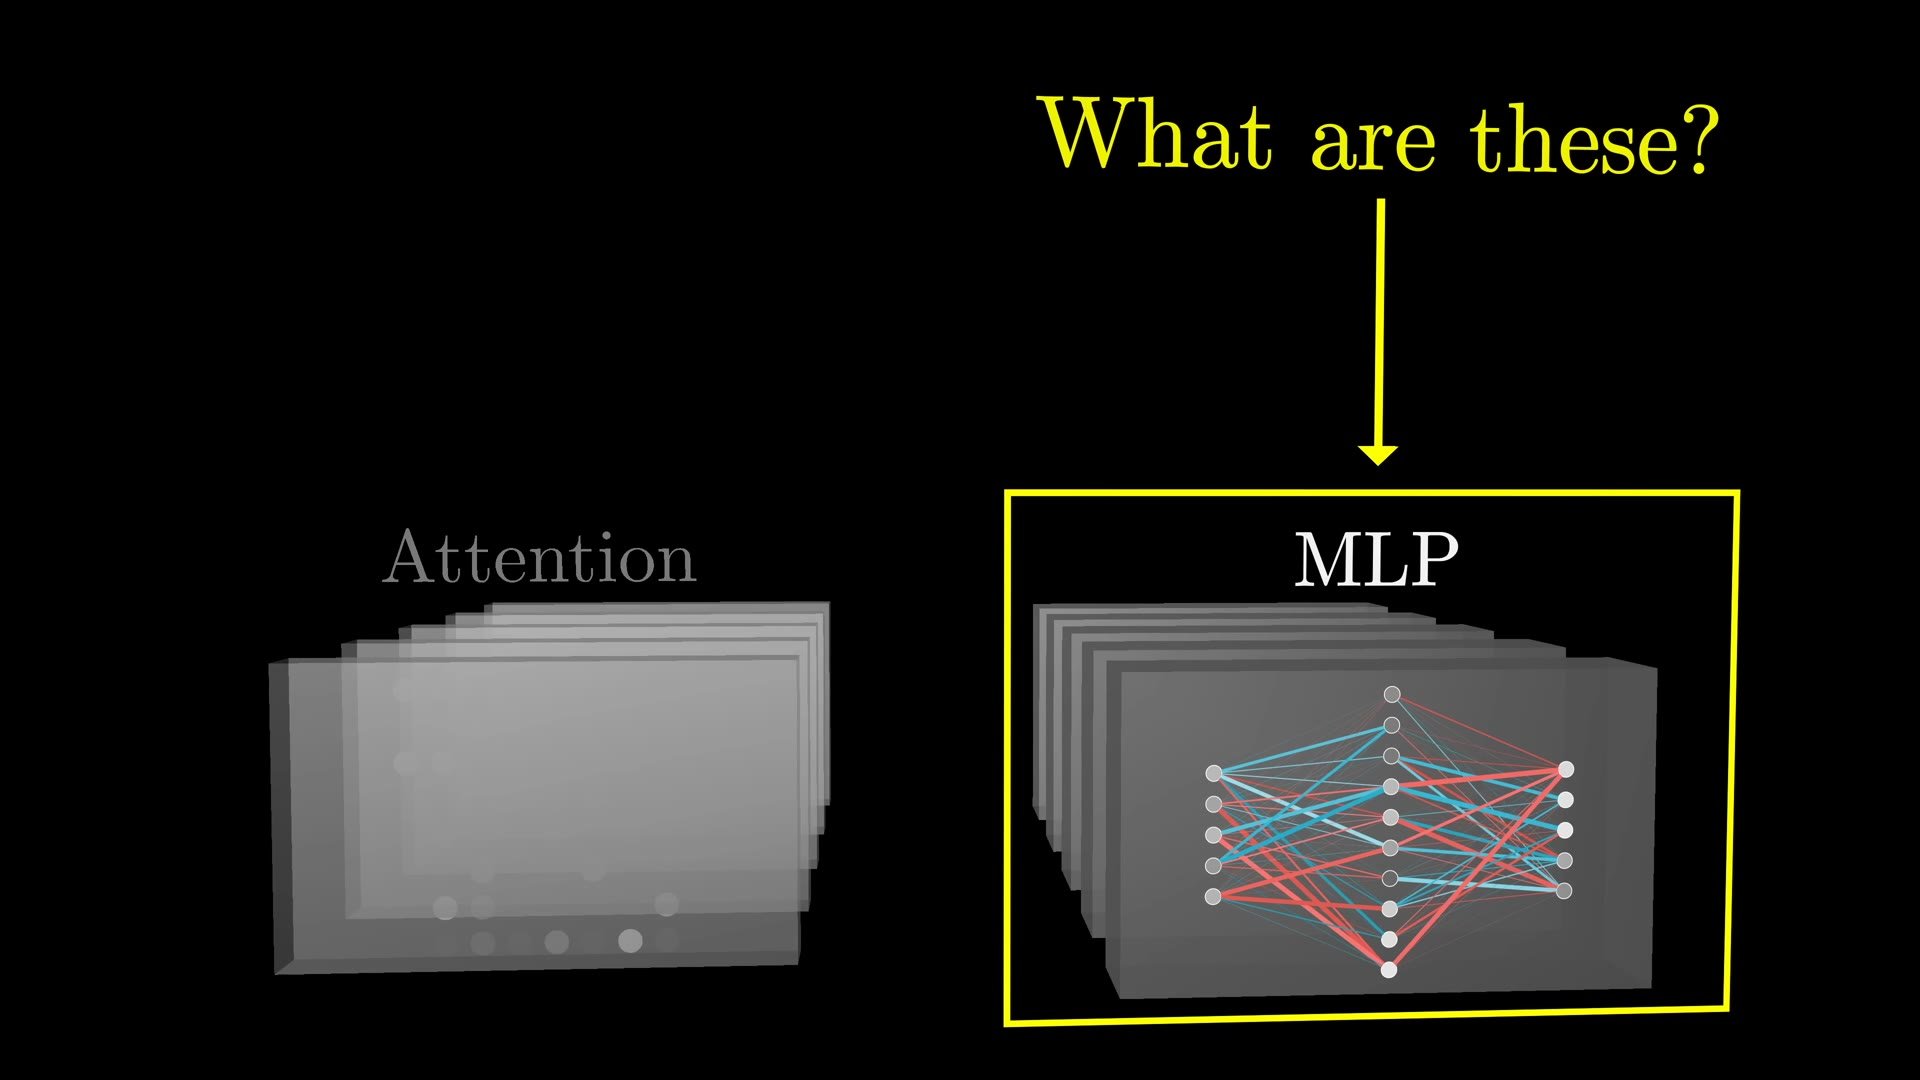
\includegraphics[width=\linewidth]{ch7_flow_mlp.jpg}\\ \bbb
    \column{0.42\textwidth}
    \vskip 6pt
    After attention, every token goes through the \textbf{same} small network, \textbf{alone}:
    no token sees another inside the MLP.
    \vskip 6pt
    It is the network from [41]: a linear layer, a nonlinearity, a linear layer.
    \vskip 6pt
    \keybox{Attention: tokens talk. MLP: each token thinks on its own.}
  \end{columns}
\end{frame}

\begin{frame}{A direction is a question}
  \begin{columns}[T]
    \column{0.56\textwidth}
    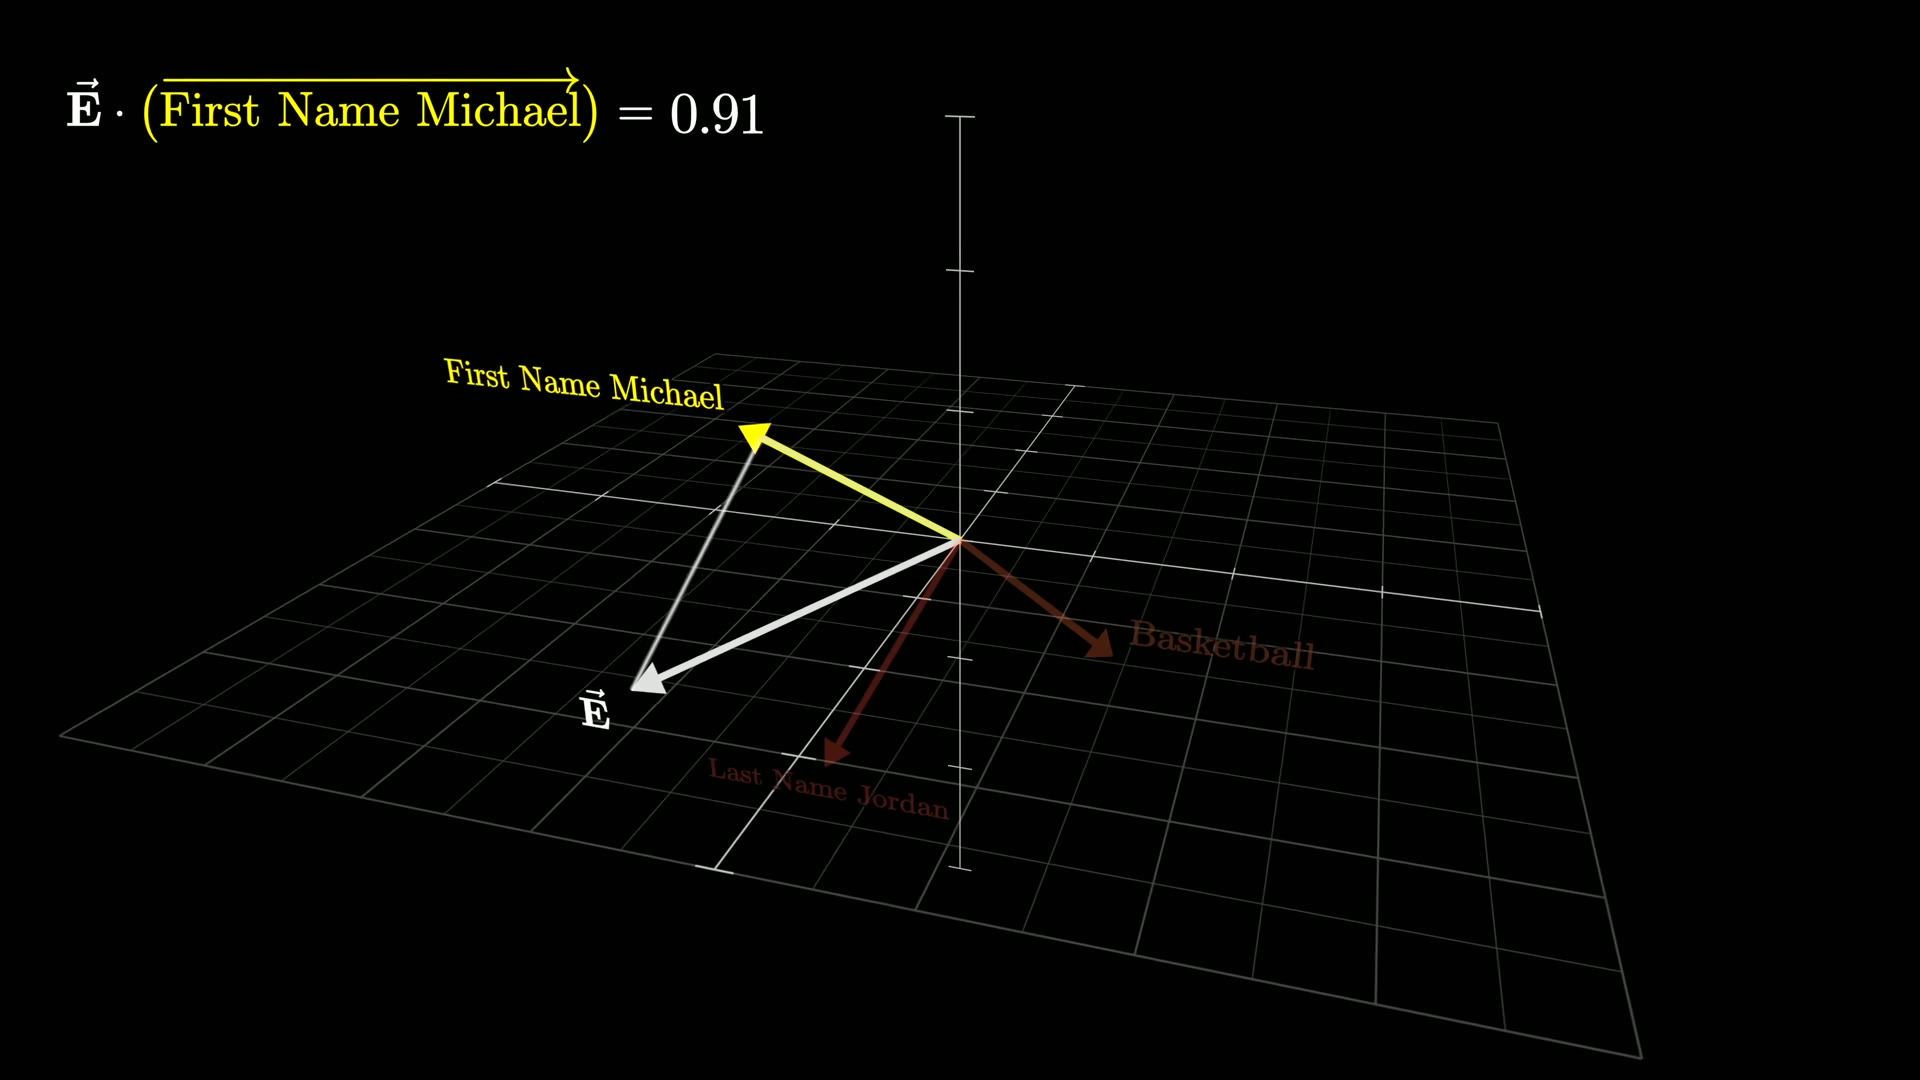
\includegraphics[width=\linewidth]{ch7_direction_dotprod.jpg}\\ \bbb
    \column{0.42\textwidth}
    \vskip 6pt
    LLM-2: directions in the vector space carry meaning. The dot product with a direction
    measures \emph{how much} of that idea a vector holds.
    \vskip 6pt
    Here: how much ``first name Michael'' is in this token's vector? $0.91$: a lot.
  \end{columns}
\end{frame}

\begin{frame}{Up-projection: each row asks a question}
  \begin{columns}[T]
    \column{0.56\textwidth}
    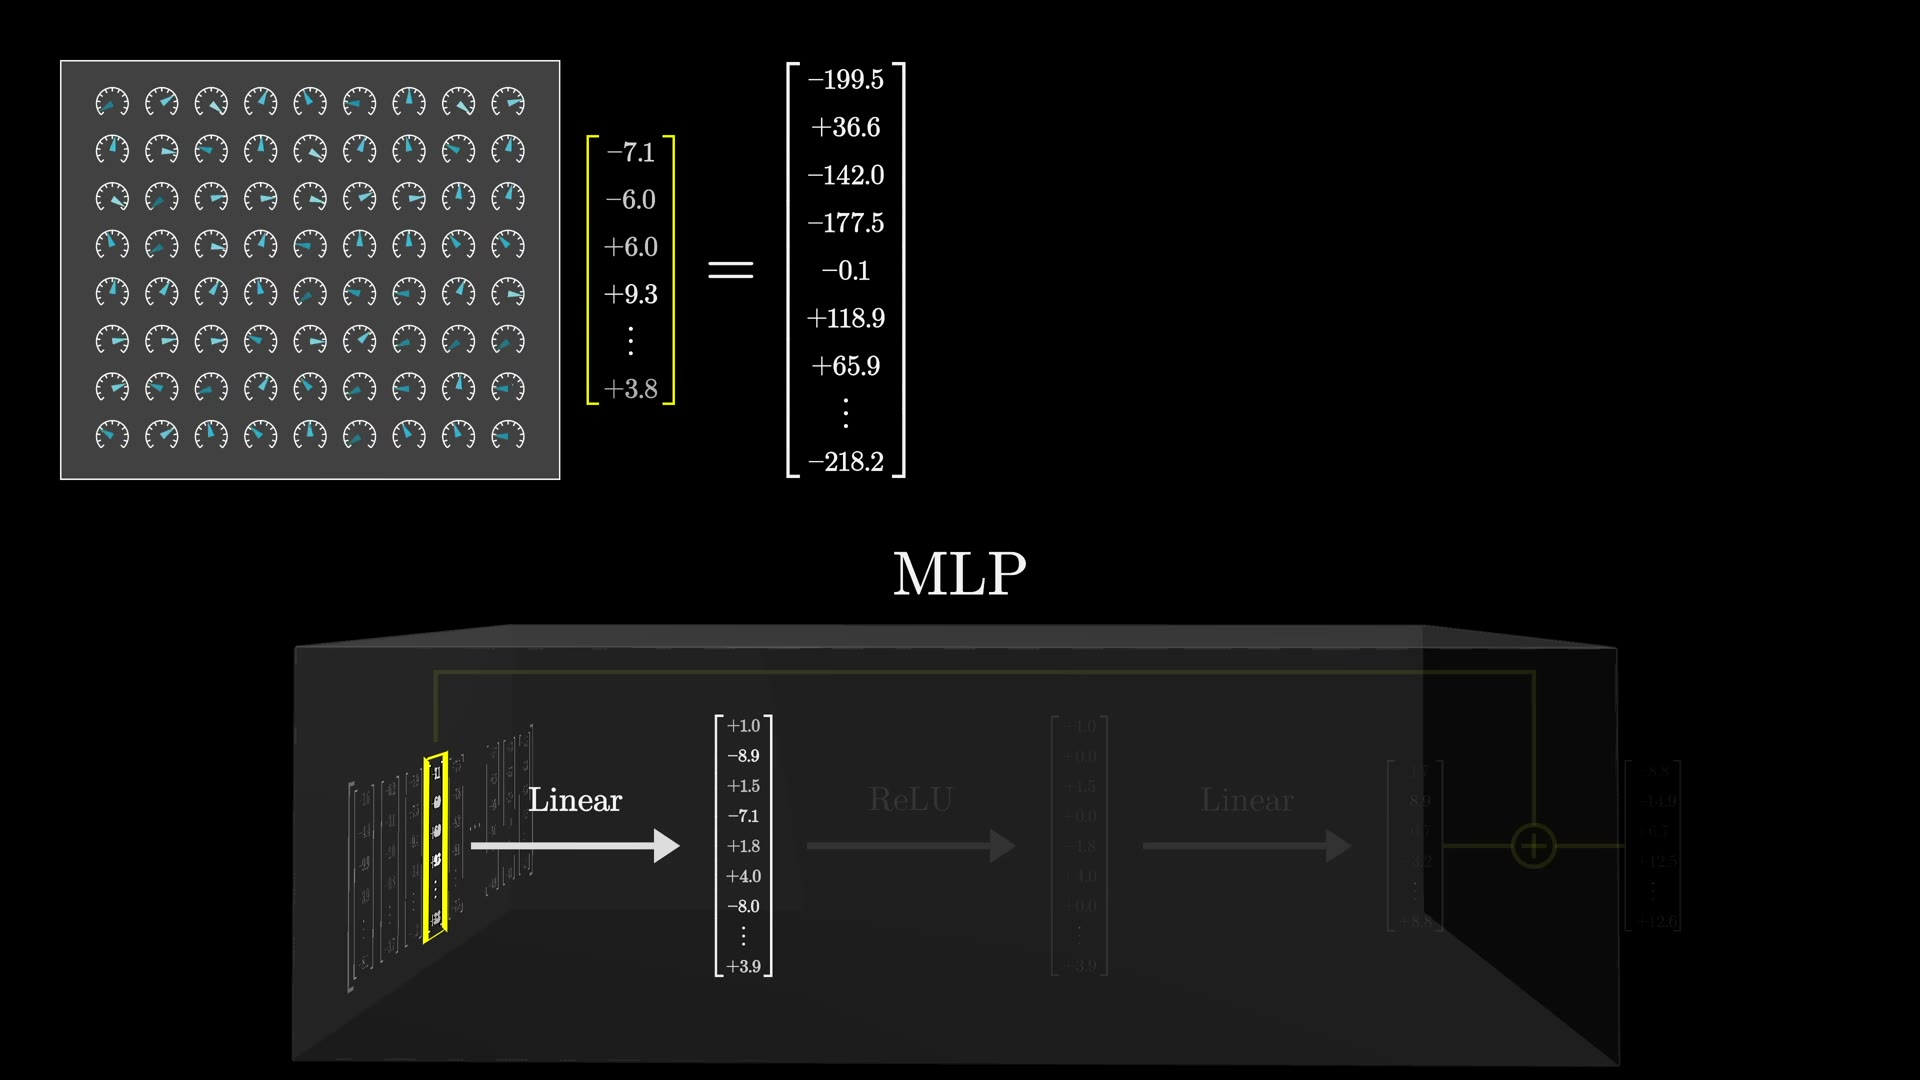
\includegraphics[width=\linewidth]{ch7_upproj_rows.jpg}\\ \bbb
    \column{0.42\textwidth}
    \vskip 6pt
    The first layer computes $W_{\text{up}}\,\mathbf{x} + \mathbf{b}$. Each \textbf{row} of
    $W_{\text{up}}$ is one such question, a dot product with one direction; the bias is a
    threshold.
    \vskip 6pt
    GPT-2 asks \textbf{3{,}072} questions per token: four times its 768 numbers (the 2017
    paper's ratio, kept since: more questions per token).
  \end{columns}
\end{frame}

\begin{frame}{ReLU makes an AND gate}
  \begin{columns}[T]
    \column{0.56\textwidth}
    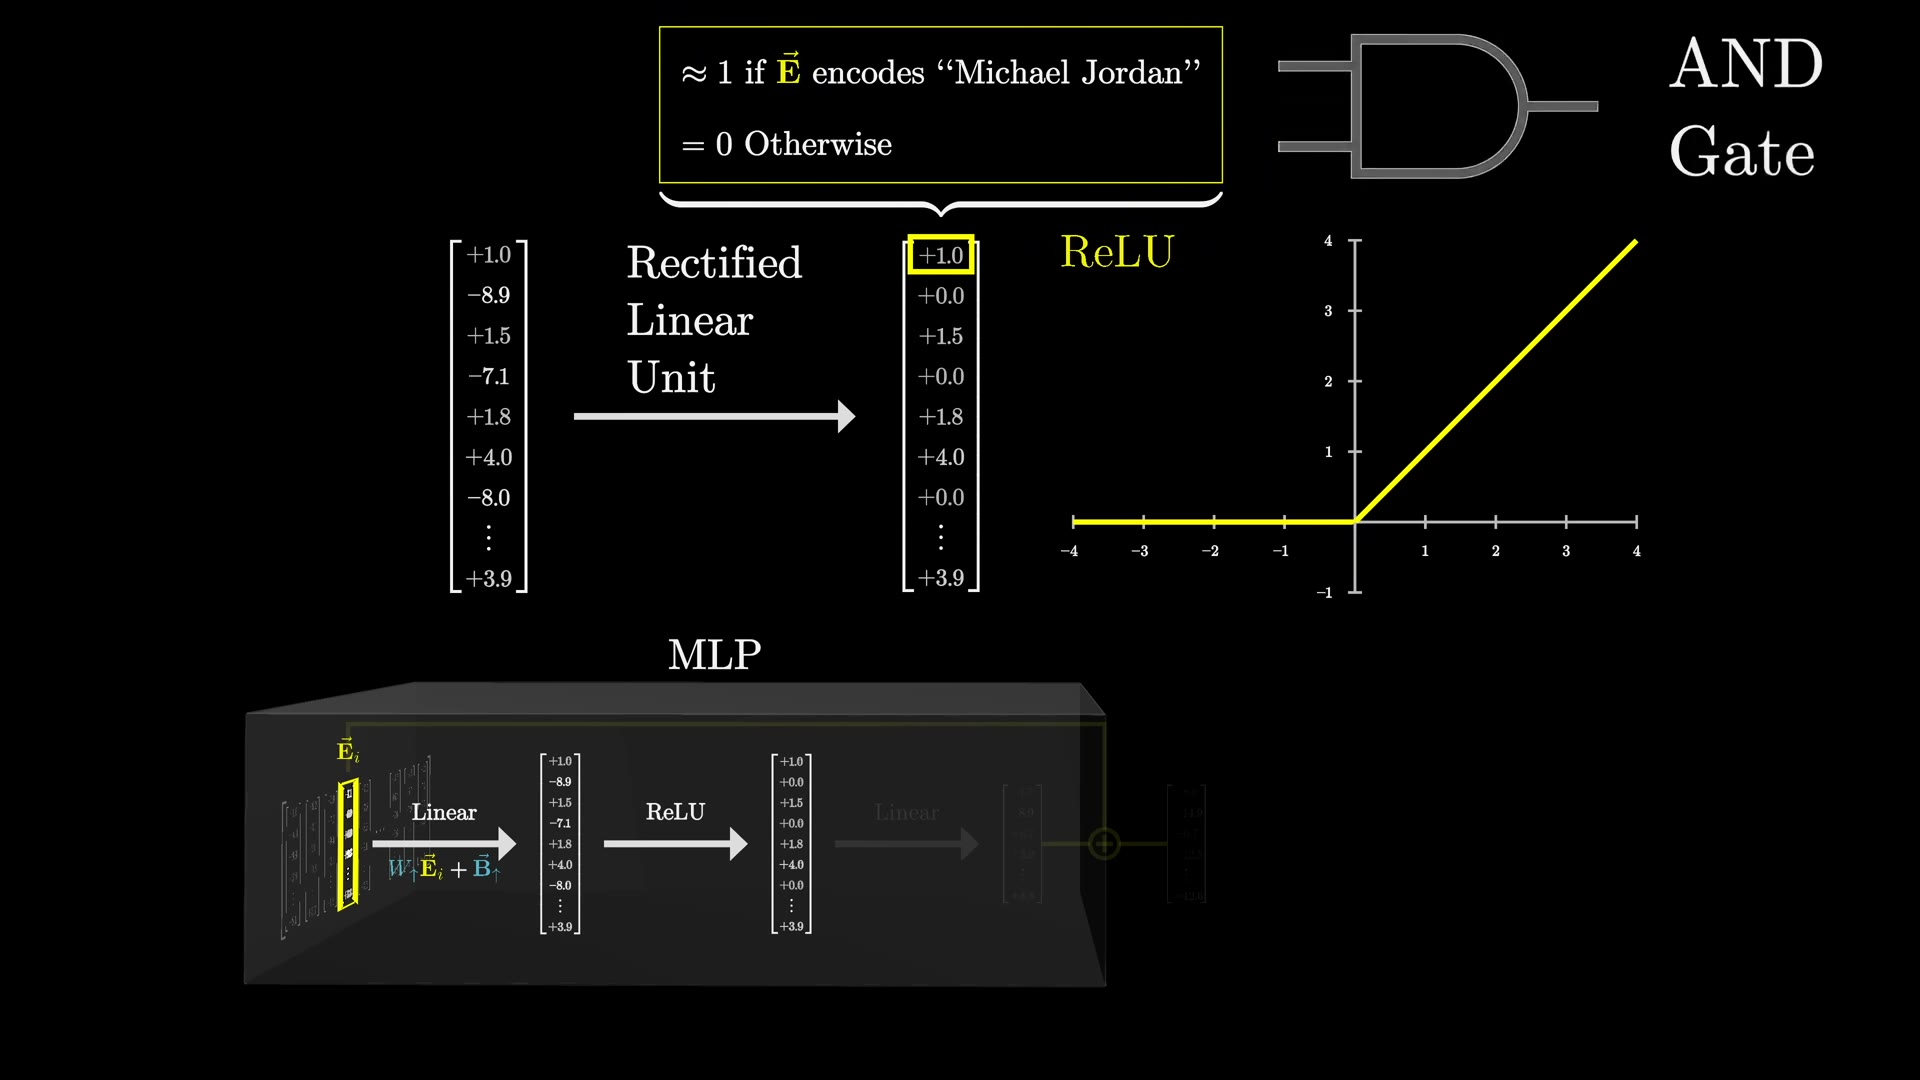
\includegraphics[width=\linewidth]{ch7_relu_andgate.jpg}\\ \bbb
    \column{0.42\textwidth}
    \vskip 6pt
    Ask ``first name Michael'' $+$ ``last name Jordan'', with bias $-1$: the sum is positive only
    if \textbf{both} are there.
    \vskip 6pt
    ReLU sets everything negative to 0. What is left is a neuron that fires on ``Michael AND
    Jordan'' and stays silent otherwise.
    \vskip 6pt
    {\footnotesize GPT-2 actually uses GELU, a smoothed ReLU (slightly negative instead of exactly
    0 below zero); the gate works the same way.}
  \end{columns}
\end{frame}

\begin{frame}{Down-projection: each column adds something}
  \begin{columns}[T]
    \column{0.56\textwidth}
    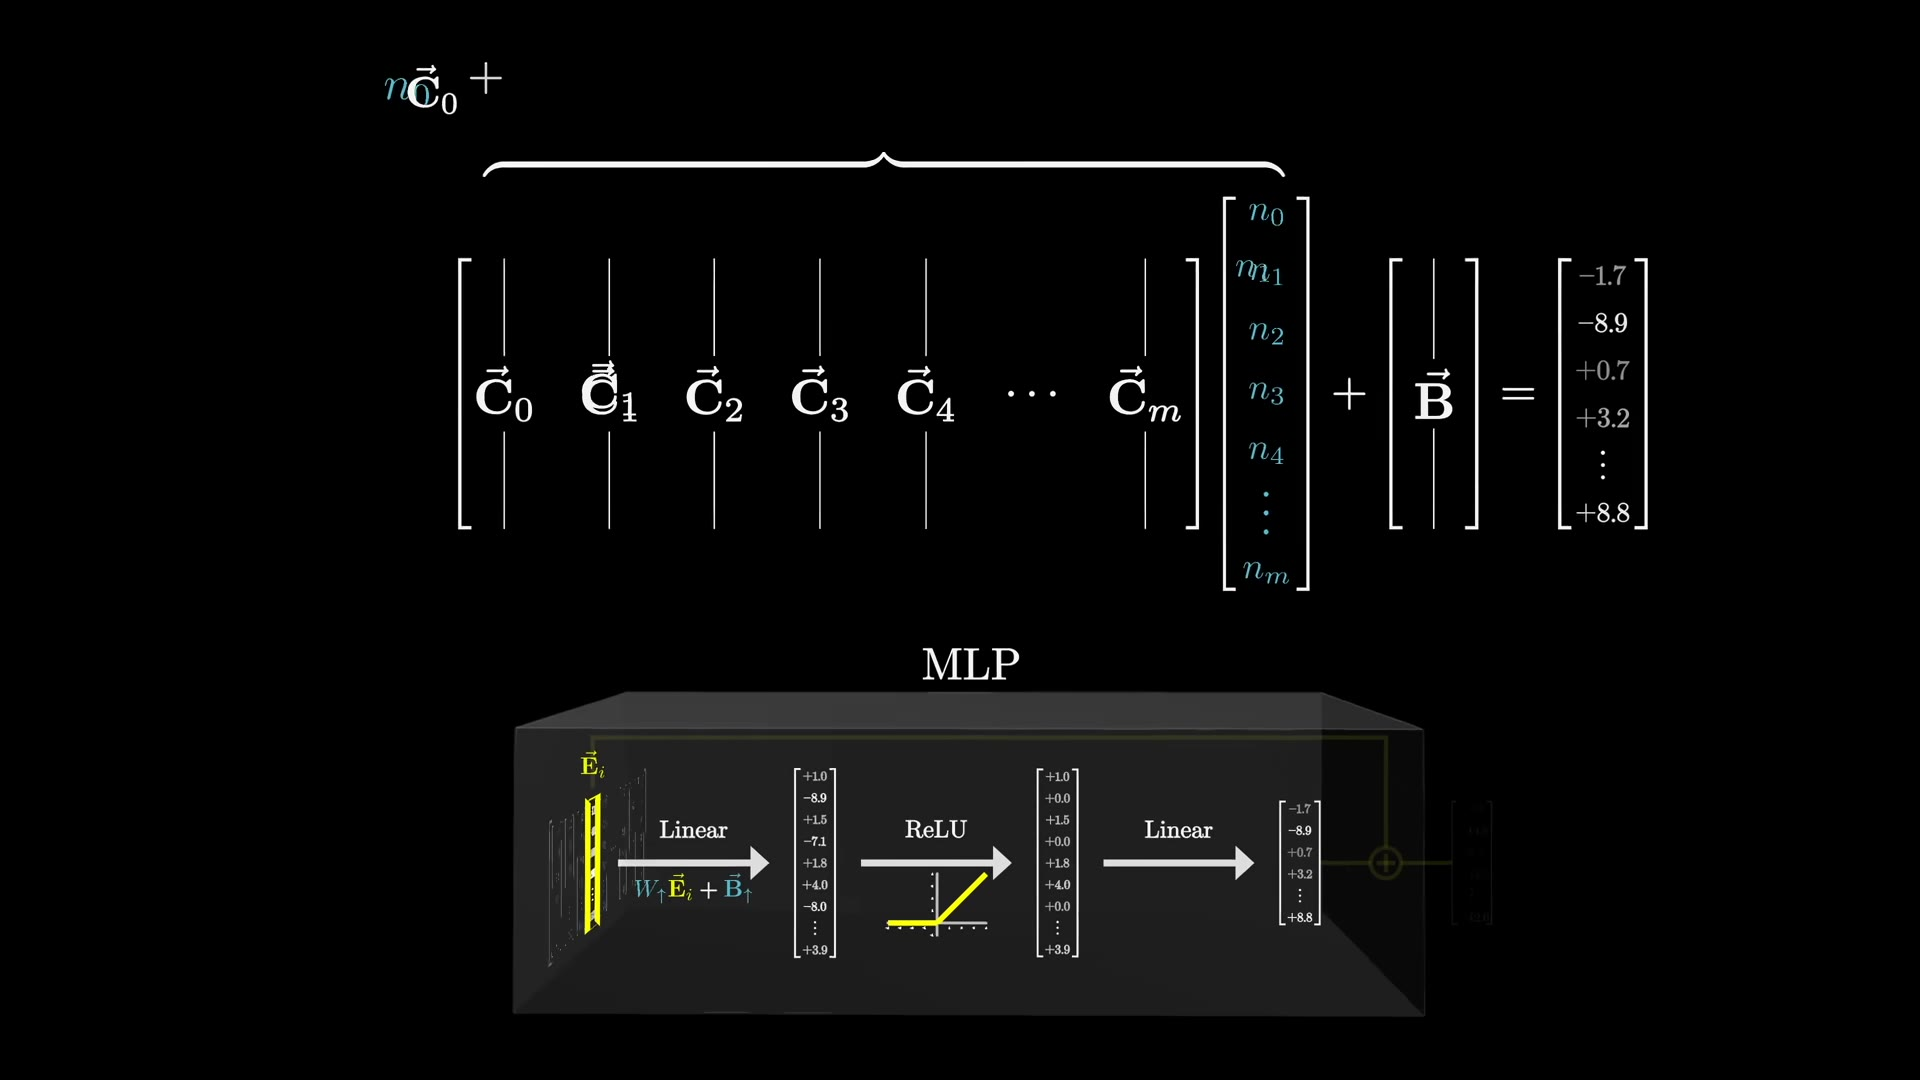
\includegraphics[width=\linewidth]{ch7_downproj_columns.jpg}\\ \bbb
    \column{0.42\textwidth}
    \vskip 6pt
    The second layer maps the 3{,}072 neuron values back to 768 numbers. Each \textbf{column} of
    $W_{\text{down}}$ is a direction; a neuron that fires adds its column into the stream.
    \vskip 6pt
    The ``Michael Jordan'' neuron's column can point toward ``basketball''. The fact is in the
    weights.
  \end{columns}
\end{frame}

\begin{frame}{By hand: a neuron on creature}
  \begin{columns}[T]
    \column{0.5\textwidth}
    \small
    Creature after LLM-3: $(0,\ 0.47,\ 0.47,\ 2.13)$, plus a fifth slot, \textbf{cute}, that every
    word left at 0 (real vectors: 768 slots, most unnamed).
    \vskip 3pt
    Row of $W_{\text{up}}$: $(0, 1, 0, 0.5, 0)$, bias $-1.2$, so the neuron is
    $\mathrm{ReLU}(\text{fluffy} + 0.5\,\text{noun} - 1.2)$:
    \begin{itemize}
      \item this creature: $0.47 + 1.065 - 1.2 = \mathbf{0.335}$
      \item plain creature $(0,0,0,2)$, fluffy alone: $-0.2 \to 0$; blue alone: $-1.2 \to 0$
    \end{itemize}
    Column of $W_{\text{down}}$: $(0, 0, 0, 0, 3)$, so it writes $3 \times 0.335 = 1.0$ into cute.
    \column{0.48\textwidth}
    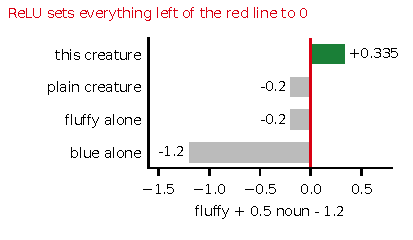
\includegraphics[width=\linewidth]{blk_neuron.pdf}
  \end{columns}
  \vskip 4pt
  \takebox{It fires on ``fluffy AND creature'' - possible only because attention first brought
  fluffy into creature's vector (LLM-3), as with Michael and Jordan. Creature now carries a
  feature no word had.}
\end{frame}

\bbbcap{ch7_mlp_full.jpg}{The whole MLP: linear, ReLU, linear, then add the result back into the
stream. The same weights for every token.}

\begin{frame}{Two thirds of the weights}
  \begin{center}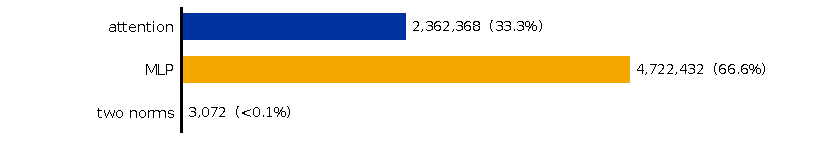
\includegraphics[width=0.9\linewidth]{blk_params_block.pdf}\end{center}
  \vskip -2pt
  {\small One GPT-2 block, counted from its weight file: the MLP holds \textbf{66.6\%}. 3Blue1Brown
  counts the same share for GPT-3. Last lecture was about the smaller half.}
  \vskip 6pt
  \watchbox{Size is room, not proof: having most of the weights does not show the facts are
  there. The evidence is next.}
\end{frame}

\begin{frame}{Why the MLP? The evidence}
  \vskip 4pt
  \begin{itemize}
    \item \textbf{Causal tracing} \paper{(Meng et al., NeurIPS 2022)}: run the prompt clean, then
      again with noise added to the subject's tokens. Copy one hidden state (one token's vector
      after one layer) from the clean run into the noisy one at a time, and see which brings the
      right answer back.
      In GPT-2 XL the decisive states are the \textbf{mid-layer MLPs at the subject's last
      token}; attention later carries the result to where the answer is written. Editing one of
      those MLPs changes the fact.
    \item \textbf{Key-value memories} \paper{(Geva et al., EMNLP 2021)}: MLP rows fire on
      recognisable input patterns, and their columns push the prediction toward related
      words - rows ask, columns add, as above.
    \item \textbf{Frequency} \paper{(Kandpal et al., ICML 2023)}: models answer worse about
      people and things that are rare in their training text.
  \end{itemize}
  \vskip 6pt
  \keybox{Back to the cold open: a neuron that fires on ``Lionel AND Messi'' can add a
  ``football'' direction - the cute neuron's mechanism. Mkhitaryan, 7 rare pieces, apparently
  never got one in GPT-2 small.}
\end{frame}

\begin{frame}{Edit one MLP, move the Eiffel Tower}
  \begin{itemize}
    \item If a fact sits in a mid-layer MLP, rewriting that MLP should rewrite the fact. Meng et
      al.'s \textbf{Rank-One Model Editing} (ROME) does it with one small change to one MLP matrix
      (rank one: a column times a row).
    \item Their demo on GPT-J: insert ``The Eiffel Tower is located in the city of Rome.''
    \item Then ask in words the edit never saw. ``You can get from Berlin to the Eiffel Tower
      by'' $\to$ ``train. You can take the ICE from Berlin Hauptbahnhof to Rome Centrale.''
      ``The Eiffel Tower is right across from'' $\to$ ``the Vatican.''
  \end{itemize}
  \vskip 6pt
  \keybox{The new fact carries over to questions phrased differently - what you would expect if
  it is stored in one place and read from there.}
  \vskip 2pt
  \src{Meng et al. (NeurIPS 2022); the Eiffel Tower example is on the project page,
  rome.baulab.info. The paper's own examples edit the Space Needle and Pierre Curie.}
\end{frame}

\begin{frame}{More facts than dimensions?}
  \begin{columns}[T]
    \column{0.52\textwidth}
    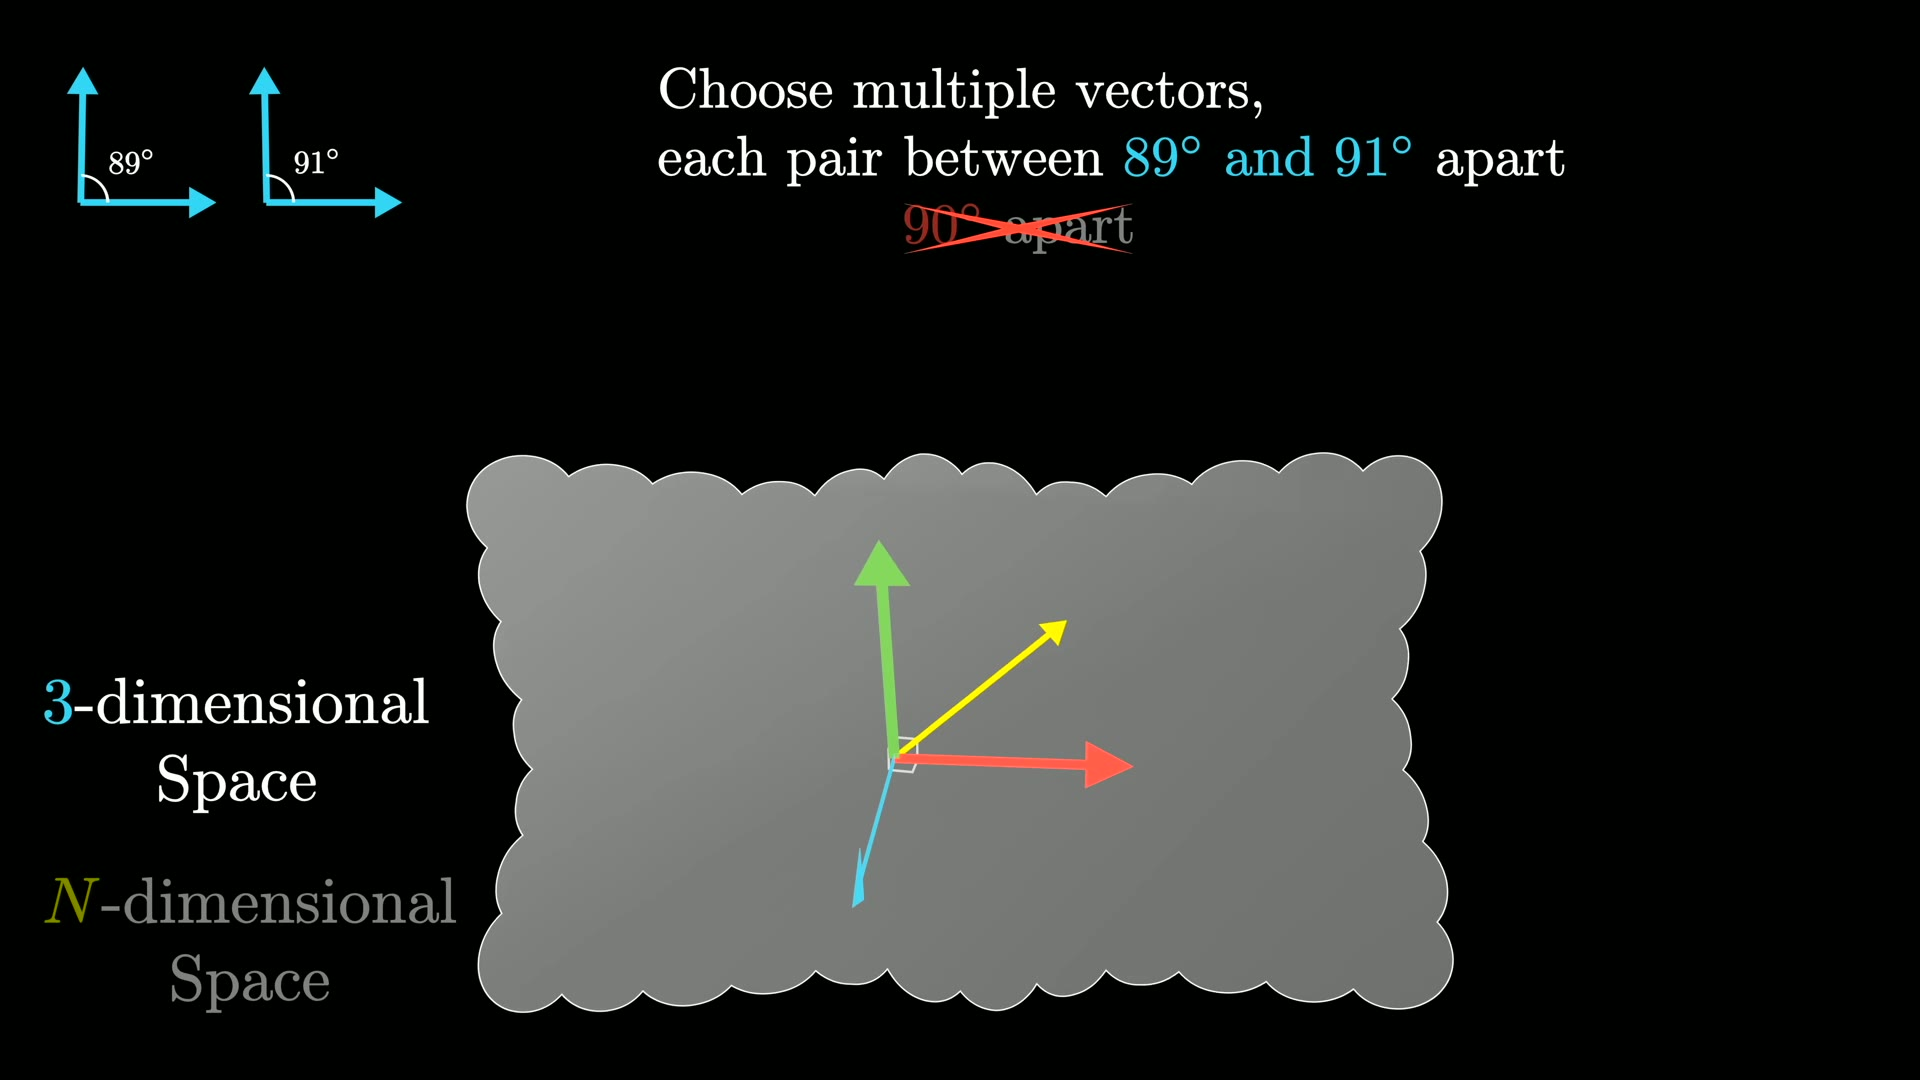
\includegraphics[width=\linewidth]{ch7_nearly_perp.jpg}\\ \bbb
    \column{0.46\textwidth}
    \vskip 6pt
    768 numbers per token, yet a model knows far more than 768 things. How?
    \vskip 6pt
    In many dimensions, directions do not have to be exactly perpendicular to stay out of each
    other's way: nearly perpendicular (89 to 91 degrees) is enough, and you can fit far more of
    those than there are dimensions.
    \vskip 6pt
    \watchbox{This idea - many features squeezed into fewer dimensions - is called
    \textbf{superposition}. So a clean ``Michael Jordan neuron'' is a teaching picture: real
    neurons mostly mix several features. More in the interpretability chapter.}
  \end{columns}
\end{frame}

\bbbcap{ch7_jl_lemma.jpg}{Johnson-Lindenstrauss: the number of nearly perpendicular directions grows
exponentially with the dimension.}

\begin{frame}{Turn one direction up: Golden Gate Claude}
  \begin{itemize}
    \item Anthropic (May 2024) pulled millions of such directions, called \textbf{features}, out
      of the residual stream of Claude 3 Sonnet (the stream every MLP reads from and writes to),
      with a sparse autoencoder. One fired on the Golden Gate Bridge.
    \item They clamped that one direction at 10 times its usual maximum and asked ``what is your
      physical form?''. Claude: ``I am the Golden Gate Bridge\ldots{} my physical form is the
      iconic bridge itself.''
    \item The usual answer: ``I have no physical form, I am an AI model.'' Golden Gate Claude was
      online for 24 hours as a research demo.
  \end{itemize}
  \vskip 6pt
  \keybox{A concept is a direction, and behaviour follows what is written into the stream.
  Features, superposition and sparse autoencoders: the interpretability chapter.}
  \vskip 2pt
  \src{Anthropic, ``Golden Gate Claude'' (23 May 2024); Templeton et al. (2024), ``Scaling
  Monosemanticity'', Transformer Circuits Thread.}
\end{frame}

% ============================================================ SECTION 3
\section{The block}
\sectiontransition{The block}{What you actually stack.}

\begin{frame}{The Transformer block}
  \begin{columns}[T]
    \column{0.42\textwidth}
      \vskip -4pt
      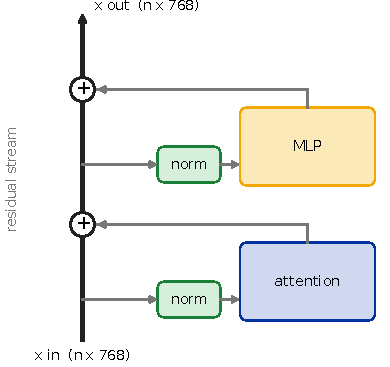
\includegraphics[width=\linewidth]{blk_block.pdf}
    \column{0.56\textwidth}
      \vskip 8pt
      {\small
      \textbf{Attention}: tokens exchange information. The \emph{only} place in the block where
      tokens see each other.
      \vskip 5pt
      \textbf{MLP}: each token alone; two thirds of the weights.
      \vskip 5pt
      \textbf{Norm} before each, and the result \textbf{added back}: LayerNorm from [44], the
      residual connection from [49].}
      \vskip 6pt
      \keybox{Every piece but attention is something you already met. GPT-2's order: norm,
      sublayer, add.}
  \end{columns}
\end{frame}

\begin{frame}{The residual stream is the real object}
  \vskip 6pt
  Read the block as a \textbf{stream} of token vectors running straight through the network, and
  each sublayer \emph{writing an update into it}:
  \vskip 8pt
  \begin{center}
    $\mathbf{x} \leftarrow \mathbf{x} + \text{Attention}\big(\text{LN}(\mathbf{x})\big)$
    \qquad then \qquad
    $\mathbf{x} \leftarrow \mathbf{x} + \text{MLP}\big(\text{LN}(\mathbf{x})\big)$
    \qquad {\small (LN = LayerNorm)}
  \end{center}
  \vskip 6pt
  Unroll it over all $L$ sublayers, with $\mathbf{u}_i$ the update sublayer $i$ writes:
  \[
    \mathbf{x}_L = \mathbf{x}_0 + \mathbf{u}_1 + \mathbf{u}_2 + \cdots + \mathbf{u}_L
  \]
  \vskip -4pt
  \takebox{The stream itself is never normalised (only once, at the very top, before the LM head:
  \mbox{LLM-5}). Each sublayer reads a normalised copy and adds a \textbf{correction}, so every
  update is still in the sum, untouched, and the gradient reaches each $\mathbf{u}_i$ directly:
  the derivative of a sum - the ResNet argument from [49]. Normalise the stream after every add
  instead, and each norm rescales everything written so far.}
  \vskip 6pt
  {\scriptsize\color{gray} GPT-2 moved the norm ``to the input of each sub-block'' (Radford et al.,
  2019). The 2017 paper normalised after the add: $\mathbf{x} \leftarrow
  \text{LN}(\mathbf{x} + f(\mathbf{x}))$.}
\end{frame}

\begin{frame}{By hand: LayerNorm on creature}
  \vskip 4pt
  LayerNorm ([44]) rescales one token's vector so its numbers have mean 0 and spread 1. Creature
  after LLM-3, $(0,\ 0.47,\ 0.47,\ 2.13)$:
  \vskip 6pt
  \begin{center}
  \begin{tabular}{ll}
    mean & $(0 + 0.47 + 0.47 + 2.13)/4 = 0.77$ \\[2pt]
    spread & $\sqrt{\tfrac{1}{4}\sum (x_i - 0.77)^2} = 0.81$ \\[2pt]
    normalised & $(x - 0.77)/0.81 = (-0.95,\ -0.37,\ -0.37,\ 1.68)$ \\[2pt]
    then & times a learned scale, plus a learned shift (1 and 0 here) \\
  \end{tabular}
  \end{center}
  \vskip 8pt
  \keybox{Each token is normalised on its own numbers - not across the batch, as BatchNorm does
  ([44]). Attention and the MLP read this copy, $(-0.95, -0.37, -0.37, 1.68)$; the stream keeps
  $(0, 0.47, 0.47, 2.13)$ and gets their update added.}
\end{frame}

\begin{frame}{Modern block recipe}
  \vskip 8pt
  The block has been tuned since 2017. Four changes you will meet in current models:
  \vskip 8pt
  \begin{center}
  \footnotesize
  \begin{tabular}{lll}
    \toprule
    \textbf{2017} & \textbf{Now} & \textbf{Why} \\
    \midrule
    norm after the add & norm first (GPT-2 already) & trains more stably; can even skip warm-up \\
    LayerNorm & \textbf{RMSNorm} & cheaper: no mean, only the spread \\
    ReLU in the MLP & \textbf{SwiGLU} & a gated MLP; better quality in Shazeer's tests \\
    MLP $4\times$ wide & $2.7\times$ wide, 3 matrices & about the same weights \\
    \bottomrule
  \end{tabular}
  \end{center}
  \vskip 6pt
  {\scriptsize\color{gray} Xiong et al., ICML 2020 (norm first); Zhang \& Sennrich, NeurIPS 2019
  (RMSNorm); Shazeer, 2020 (GLU variants). Gated: two up-projections, one multiplied into the
  other. Width: Llama 2 7B goes 4,096 $\to$ 11,008 (config.json); $3 \times 2.7 \approx 2 \times 4$.}
  \vskip 8pt
  \watchbox{None of these changes the story: attention, an MLP, norms and the residual stream.
  LLM-14 opens a 2026 model card and finds the same block.}
\end{frame}

\begin{frame}{Now stack it}
  \begin{columns}[T]
    \column{0.5\textwidth}
      \vskip -4pt
      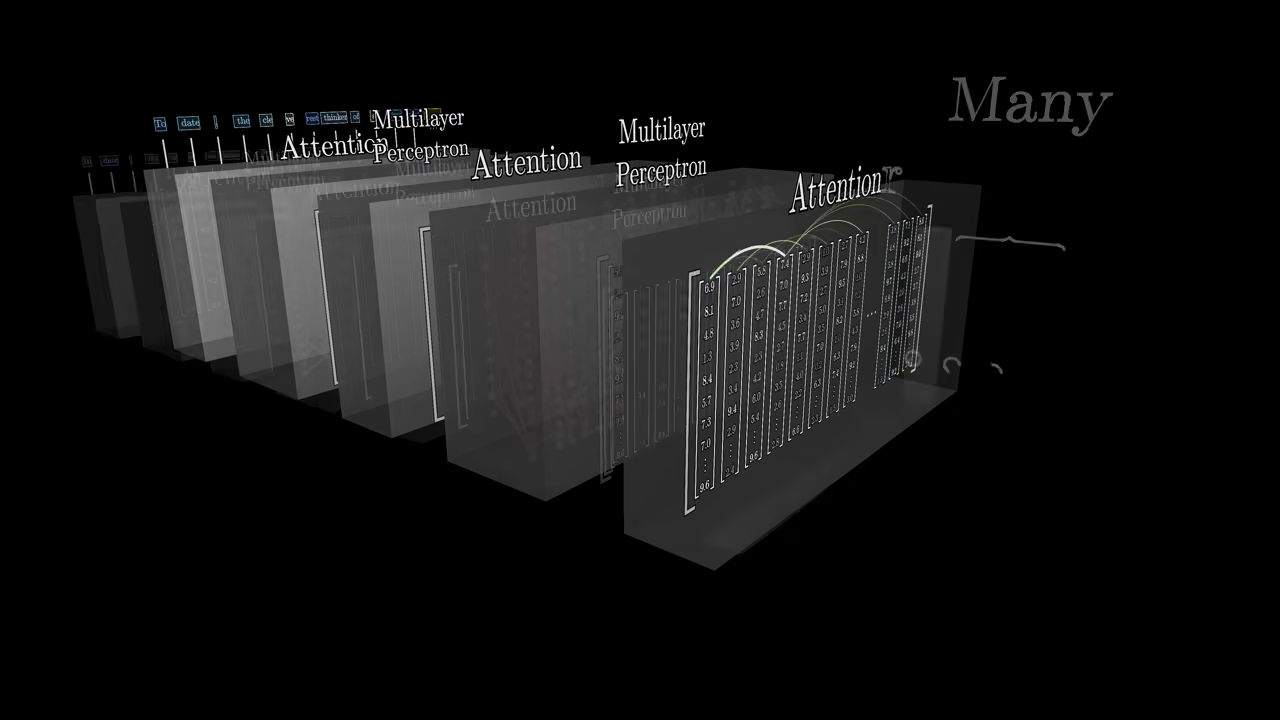
\includegraphics[width=\linewidth]{deep_stack.png}\\ \bbb
    \column{0.47\textwidth}
      \vskip 8pt
      {\small A block takes $n \times 768$ numbers in and gives $n \times 768$ out - the same
      shape, which is why blocks can be stacked. GPT-2 small stacks \textbf{12}.
      \vskip 8pt
      Each block alternates \textbf{tokens talking} (attention) with \textbf{each token thinking
      alone} (the MLP).
      \vskip 8pt
      A token's vector starts as ``the word \emph{creature}'' and, layer by layer, gathers what
      the context implies: fluffy, blue, cute, and whatever comes next.}
  \end{columns}
  \vskip 4pt
  \takebox{Same block, 12 times. That is the whole architecture. And since every layer only
  \emph{adds}, you can read the stream after any layer through the final LM head and watch the
  guess form: the ``logit lens'' (2020).}
\end{frame}

\begin{frame}{Where GPT-2's 124M live}
  \begin{center}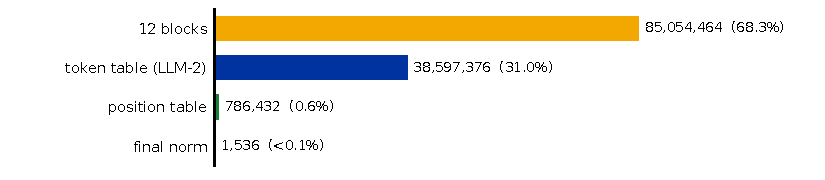
\includegraphics[width=0.94\linewidth]{blk_params_124m.pdf}\end{center}
  \vskip -2pt
  {\small $12 \times 7{,}087{,}872 = 85{,}054{,}464$ in the blocks; the token table (LLM-2's 31\%);
  1{,}024 learned positions; one final norm. Total \textbf{124{,}439{,}808}, read from the weight
  file.}
  \vskip 6pt
  \keybox{Two thirds of every block is MLP, and the blocks are two thirds of the model. Attention,
  the star of LLM-3, is under a quarter of GPT-2 (22.8\%).}
\end{frame}

% ============================================================ RECAP
\begin{frame}{Recap}
  \vskip 4pt
  \small
  \begin{itemize}
    \item \textbf{Many heads}: $h$ questions at once, each in a smaller space (GPT-2: $12 \times
      64 = 768$), mixed by $W_O$. Real heads: one looks one token back, one sends creature to
      fluffy, many park on the first token.
    \item \textbf{Heads team up}: a previous-token head plus an induction head copy
      \ldots A B \ldots A $\to$ B from the prompt. Sinks went from quirk to design in 2025.
    \item \textbf{Still blind to order}: one head or twelve, so positions come in before the first
      layer (LLM-2).
    \item \textbf{The MLP}: rows ask, ReLU gates, columns add. A neuron can fire on ``fluffy AND
      creature'', and facts like Messi's sport seem to live here: edit one MLP and the Eiffel
      Tower moves to Rome. Two thirds of every block.
    \item \textbf{The block}: norm, attention, add; norm, MLP, add. The stream is never
      normalised; every sublayer writes a correction.
    \item \textbf{The mask} (LLM-3) sits in every attention layer: no block reads the future.
  \end{itemize}
\end{frame}

\begin{frame}{Next on the map}
  \begin{center}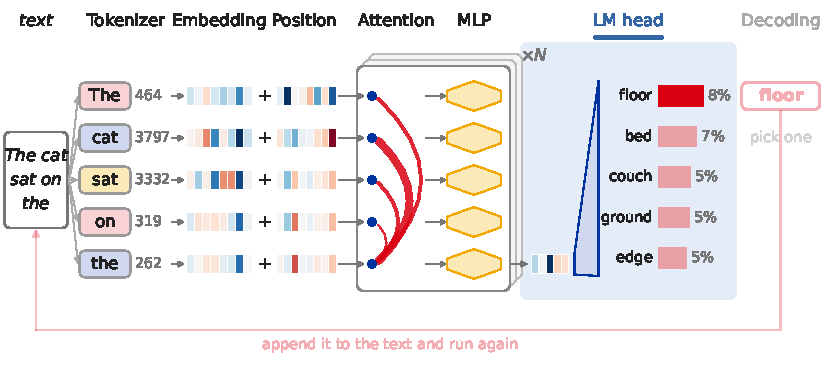
\includegraphics[width=\linewidth]{roadmap_transformers_pass.pdf}\end{center}
  \vskip -2pt
  {\small Next (LLM-5): what comes out at the far end, and three ways to wire the same block.}
\end{frame}

\begin{frame}{Sources \& further reading}
  \footnotesize
  \begin{itemize}
    \item \textbf{Watch:} 3Blue1Brown (2024),
      \link{https://www.youtube.com/watch?v=9-Jl0dxWQs8}{How might LLMs store facts \textbar{} Deep
      Learning Chapter 7}; Karpathy (2023), \link{https://youtu.be/kCc8FmEb1nY?t=4919}{Let's build
      GPT: from scratch, in code, spelled out.} \textbf{Play:}
      \link{https://poloclub.github.io/transformer-explainer/}{Transformer Explainer}.
    \item Vaswani et al. (2017), ``Attention Is All You Need'', NeurIPS; Radford et al. (2019),
      ``Language Models are Unsupervised Multitask Learners'' (GPT-2).
    \item Olsson et al. (2022), ``In-context Learning and Induction Heads'', Transformer Circuits
      Thread.
    \item Xiao et al. (2024), ``Efficient Streaming Language Models with Attention Sinks'', ICLR;
      Miller (2023), ``Attention Is Off By One'' (blog); OpenAI (2025), gpt-oss model card; Qiu et
      al. (2025), ``Gated Attention for Large Language Models'', NeurIPS.
    \item Geva et al. (2021), ``Transformer Feed-Forward Layers Are Key-Value Memories'', EMNLP;
      Meng et al. (2022), ``Locating and Editing Factual Associations in GPT'', NeurIPS; Kandpal et
      al. (2023), ``Large Language Models Struggle to Learn Long-Tail Knowledge'', ICML.
    \item Templeton et al. (2024), ``Scaling Monosemanticity'', Transformer Circuits Thread;
      nostalgebraist (2020), ``interpreting GPT: the logit lens'', LessWrong.
    \item Xiong et al. (2020), ``On Layer Normalization in the Transformer Architecture'', ICML;
      Zhang \& Sennrich (2019), ``Root Mean Square Layer Normalization'', NeurIPS; Shazeer (2020),
      ``GLU Variants Improve Transformer'', arXiv.
  \end{itemize}
\end{frame}

\end{document}

% ============================================================================
% Provenance
%
% PLAN: llms/ATTENTION_CHAPTER_PLAN.md, section "L25", approved by the instructor
% 2026-07-19. Frame order follows that outline; the optional "modern block recipe" frame was
% kept rather than cut.
%
% SOURCES:
%   - misc/dl4nlp/02_transformers.tex - multi-head, positional encoding, the block, and the
%     modern-variant table were adapted from it (already in the house palette).
%   - 3Blue1Brown Ch5/Ch6, transcripts in research/, frames in fig/borrowed/3b1b/ with a
%     manifest. Used: multihead.png, attn_mlp_flow.png, deep_stack.png, single_head_full.png.
%     Credit line only, per the instructor's 2026-07-21 decision (no licence tag).
%   - Vaswani et al. (2017) for the PE formula; the architecture figure itself is used in L26.
%
% FIGURES - py_src/l25_l26_figs.py and py_src/l25_real_attention.py:
%   REAL (every number quoted on a slide comes from these scripts' logs):
%     l25_permutation    - the same three tokens in two orders give per-token outputs differing
%                          by 1.1e-16 without positional encoding, and 1.797 with it. The script
%                          RAISES if the no-PE gap exceeds 1e-9, so the deck's central claim in
%                          section 2 cannot silently become false.
%     l25_pe_heatmap     - the sinusoidal matrix, computed from the formula on the slide.
%     l25_pe_dotprod     - PE similarity depends on offset not absolute position; the curves for
%                          positions 10/25/40 agree to within 0.0000.
%     l25_causal_mask    - masked attention pays exactly 0.000 to future tokens; script asserts it.
%     l25_real_heads     - REAL attention weights pulled from intfloat/multilingual-e5-small
%     l25_head_entropy     (12 layers x 12 heads) on the 3b1b running sentence, so the chapter
%                          keeps one example from L24's single head through to multi-head.
%                          Layer 6: sharpest head 1 (entropy 0.92), most diffuse head 0 (1.85).
%   ILLUSTRATIVE (labelled "schematic" on the figure itself):
%     l25_block          - the block as a data-flow diagram.
%
% DELIBERATE CHOICES:
%   - The permutation result is the section-2 predict-first payoff. It is stated as a proof
%     ("not slightly different - identical") because it is one: the mechanism has no term in i
%     or j, which the following frame spells out.
%   - The "what heads learn" frame carries an explicit warning that the labels are our
%     interpretation, not measured. The measured claim is the entropy spread on the frame before.
%   - RoPE and ALiBi are named in one line and not derived, per the plan.
%
% NOT DONE:
%   - No homework frame (house rule: homework lives on the chapter .qmd).
%   - Cross-attention is deferred to L26, where it belongs with the encoder-decoder family.
%   REVISION 2026-10-04: two "Where we are" frames after the title (one forward pass; the life
%   of a model) and "Next on the map" before the closing frame (fig/roadmap_block_pass/_life.pdf,
%   roadmap_transformers_pass.pdf from py_src/llm_roadmap.py; DECISIONS #67).
%   RENAMED 2026-10-05 (DECISIONS #71, the chapter renumbered in teaching order): L25_transformer_block.tex -> LLM4_transformer_block.tex.
%   Labels in the body were renumbered by script; this provenance block keeps the old names.
%   RESTRUCTURED 2026-10-05 (critique, two interview rounds and follow-ups, and the outline in
%     LLM4_transformer_block_OUTLINE.md and LLM_CHAPTER_PLAN.md). Cold open on GPT-2's real fact
%     completions (Messi stored; Mkhitaryan missing; Ella Fitzgerald and Elliott Smith missed to
%     different degrees - people picked by the instructor after three probe runs). Sections: Many
%     heads; The MLP: where facts live (the 3b1b chapter-7 stills extracted in July for this, now
%     used); The block (GPT-2's norm-first order). Cut: the Position section except one proof frame
%     (LLM-2 owns position, #68; the sinusoid frames carried wrong extrapolation claims), the
%     "Where we got to" recap, attn_mlp_flow, the "You can now build one" ending; the e5 real heads.
%     New, from py_src/block_figs.py (toy numbers asserted; --gpt2 = one run of the cached GPT-2:
%     probes, name tokens, attention of every head on the creature sentence, parameter counts from
%     the safetensors header): blk_fact_probes, blk_two_heads (one number per head), blk_gpt2_entropy
%     and blk_gpt2_heads (layer 5 head 11 = previous token, weight 1.00; layer 6 head 2 = creature
%     -> fluffy .62; an attention-sink head; 39 of 144 heads > 90% on the first token),
%     blk_neuron (fluffy AND creature -> the new "cute" slot), blk_params_block (MLP 66.6%),
%     blk_params_124m, blk_block (norm first), blk_mask_grid. Callbacks re-pointed to the current
%     decks: LayerNorm and BatchNorm [44], residual [50], the MLP [41] (July said L14/L15/L17).
%     Notation W_Q, W_K, W_V, W_O (subscripts, as LLM-3). Sources checked: GPT-2 paper ("moved to the
%     input of each sub-block"); Xiao et al. (attention sinks), Geva et al. 2021, Meng et al. 2022,
%     Kandpal et al. 2023, Xiong et al. 2020, Zhang & Sennrich 2019, Shazeer 2020 cited from memory
%     of the papers - recheck venues before delivery.
%     Build fixes: "Stored, half-stored, missing" and "Three real heads" each split in two ("So where
%     does a fact live?", "Attention sinks" with blk_gpt2_sink, the first-token share per layer);
%     l25_permutation and l25_causal_mask (drawn 9+ in wide, text 3.6-4.7 pt on the slide) ported
%     into block_figs.py at slot size as blk_permutation (1.1e-16 reproduced, asserted) and
%     blk_causal_mask. 41 pages; 0 errors, 0 overflow, 0 footer collisions, 0 small text, 0 clipping
%     flags. No student review yet (needs the instructor's OK).
%     Self-review round (2026-10-05, instructor back): GPT-2's MLP uses GELU, not ReLU (config
%     "gelu_new") - one line on the ReLU frame; Meng et al. edited GPT-2 XL; "the first token,
%     whatever it is" narrowed to this sentence's "a"; the attention-sink reason marked as the usual
%     explanation; "attention is about a fifth of GPT-2" -> "under a quarter (22.8%)", asserted in
%     block_figs.py; "today's answer" hedged like the evidence frame; LN spelled out; the three
%     real-head titles split over two lines (they ran into each other).
%   STUDENT REVIEW 2026-10-05 (one Sonnet agent on the rendered PNGs, ~99k tokens, 88 s). Applied:
%     "attention only blends what the vectors hold" was an overclaim (W_V and W_O can write new
%     directions) - rewritten, and a new frame "Why the MLP? The evidence" (causal tracing in GPT-2 XL:
%     mid-layer MLPs at the subject's last token; key-value memories; frequency) with the Messi link,
%     while "Two thirds of the weights" now says size is room, not proof; W_O got its own by-hand
%     frame (the 4 x 2 routing matrix); the multi-head parameter count spelled out (3 x 768^2 + W_O,
%     asserted against the attention bar); the neuron's W_up row and W_down column written as
%     vectors, its chart label "this creature"; the 3b1b multi-head still flagged as GPT-3 (96
%     heads); entropy reference points; the sink's "why the first token" (the one token every later
%     token can see); why the stream stays unnormalised; LayerNorm tied to the stream; the mask
%     frame highlights fluffy's row (the one that changes); why no mask means n passes; why 4x
%     wide. Not applied: cutting the life map, Outline, MJ stills, the kinds-of-head table or the
%     modern recipe (house skeleton and interview choices); more on superposition (a teaser by
%     design). 43 pages; all checks clean.
%   STUDENT REVIEW 2 2026-10-20 (one Sonnet agent, PNGs only, ~106k tokens; DECISIONS #94).
%     Applied: "Run it h times" states the total 4 x 768^2 = 2,359,296 + 3,072 biases = the block
%     chart's 2,362,368 (asserted in block_figs.py) and what 12 heads buy over one wide head (12
%     softmax weightings per token, same weights); "The residual stream is the real object"
%     unrolls x_L = x_0 + u_1 + ... + u_L (replaces "would shrink what earlier layers wrote") and
%     names the one final LayerNorm (ln_f) before the head. Offered, not picked: a causal-tracing
%     frame, and running causal tracing on the cached GPT-2. Not raised again (rejected 10-05):
%     the MJ stills, the head table, the modern recipe, the superposition aside.
%   EXTENDED 2026-10-27 (instructor: "now similarly work on llm 3 and llm 4", after LLM-1/LLM-2).
%     New: "Before we start: two videos and a demo" (3Blue1Brown ch7, exact title; Karpathy's
%     "Let's build GPT" from 1:21:59; Transformer Explainer for the parts LLM-3 skipped); "Heads
%     team up: the induction head" (Olsson et al. 2022; toy in block_figs.py fig_induction, asserted:
%     a match scores 3 -> 0.80 on "football", 0.04 elsewhere); "From quirk to design" (Miller 2023;
%     gpt-oss's per-head sink term, model card 2.2; Qiu et al., NeurIPS 2025 best paper, first-token
%     attention 46.7% -> 4.8%); "Edit one MLP, move the Eiffel Tower" (ROME; the GPT-J example is on
%     rome.baulab.info, not in the paper, said on the slide); "Turn one direction up: Golden Gate
%     Claude" (Anthropic 23 May 2024; clamp 10x max; quotes from the post); the modern-recipe table
%     gains SwiGLU's width (Llama 2 7B 4,096 -> 11,008 from the unsloth mirror of Meta's config;
%     3 x 2.69 ~ 2 x 4); the logit lens on "Now stack it"; a Sources frame (the deck had none).
%     The sinks frame points back to LLM-2's StreamingLLM; LLM-2's points here. The venues the
%     2026-10-05 note asked to recheck (Geva EMNLP 2021, Meng NeurIPS 2022, Kandpal ICML 2023,
%     Xiong ICML 2020, Zhang & Sennrich NeurIPS 2019, Shazeer arXiv 2020) are all confirmed.
%     block_figs.py ran without --gpt2 (GPT-2's weights are not cached; it reads block_gpt2.json).
%   STUDENT REVIEW 3 2026-10-27 (one Sonnet agent, 150-dpi PNGs only, ~118k tokens; DECISIONS #101).
%     Applied: the induction head's mechanism (B's query is the current token, its keys read A's
%     note) and why it needs two layers (heads in one layer cannot read each other); causal tracing
%     spelled out (clean run, noisy run, copy one hidden state back; hidden state defined); why the
%     12 heads differ (different random starts, [41]); superposition: the clean "Michael Jordan
%     neuron" is a teaching picture; Golden Gate's directions live in the stream the MLPs read and
%     write; SwiGLU's "gated" defined in the source line. Offered, not added: one token through a
%     whole block by hand, multi-head with shapes, a causal-tracing figure, a ROME edit on the cute
%     column. Not applied: cutting the life map, the plan frame, the MJ stills, the head table, the
%     superposition still (earlier rejections).
%   MASK MOVED TO LLM-3 2026-10-28 (instructor picked "move" during the LLM-3 rework): the three
%     frames "Masking: a decoder must not read the future", "By hand: the mask on creature's grid"
%     and "Why that trick matters more than it looks" are now in LLM-3's masking section (with CLM,
%     MLM and padding); blk_causal_mask / blk_mask_grid and their code left block_figs.py. Here: a
%     callback in "Three things stand between one head and GPT-2" and in the recap.
% ============================================================================
